\documentclass[14pt]{beamer}
\usepackage[english, russian]{babel}
\usepackage[utf8x]{inputenc}
\usepackage{itmobeamer}

\usepackage{csquotes}
\usepackage{graphicx}

\graphicspath{{images/}}

\title[arXiv.org]{arXiv.org}
\author[]{Симоненко Е.А., <easimonenko@mail.ru>}
\institute[]{Университет ИТМО}
\date[]{Санкт-Петербург, 2017}

\begin{document}

\itmologoslide

\begin{darkbars}
    \begin{frame}[noheader,nologo,noframenumbering]
        \titlepage
    \end{frame}
\end{darkbars}

\begin{frame}[rulogoheader,nologo,noframenumbering]
    \itmoanothertitle
\end{frame}

\begin{darkbars}
\begin{frame}[englogoheader]{Предисловие}
\end{frame}
\end{darkbars}

\begin{frame}{Право читать}
В 1996 году Richard Stallman опубликовал свой рассказ "Право читать".

В 2000 году рассказ был переведён Сергеем Коропом на русский язык.

В 2002 году текст был дополнен автором рассказа о современном положении дел.
\end{frame}

\begin{frame}{Право читать}
Для открытых публикаций Richard Stallman использовал такой копирайт:

Verbatim copying and distribution of this entire article is permitted in any medium, provided this notice is preserved.

Разрешается копирование и распространение этой статьи любым способом без внесения изменений, при условии, что это разрешение сохраняется.

\end{frame}

\begin{frame}{Creative Commons}
Дата основания: 19 декабря 2001.

\url{http://creativecommons.org/}
\end{frame}

\begin{frame}{Creative Commons}
\begin{displayquote}
	\textit{
		Creative Commons, сокращённо CC — некоммерческая организация, которая создала бесплатные для использования типовые договоры — свободные и несвободные публичные лицензии, с помощью которых авторы и правообладатели могут выразить свою волю и распространять свои произведения более широко и свободно, а потребители контента легально и проще пользоваться этими произведениями.
	}

	\textit{-- Wikipedia}
\end{displayquote}
\end{frame}

\begin{darkbars}
	\begin{frame}[englogoheader]{arXive.org}
	\end{frame}
\end{darkbars}

\begin{frame}{arXiv.org}
\url{https://arxiv.org}

Некоммерческий научный сайт

Корнеллский университет

14 августа 1991
\end{frame}

\begin{frame}{Cornell University Library}
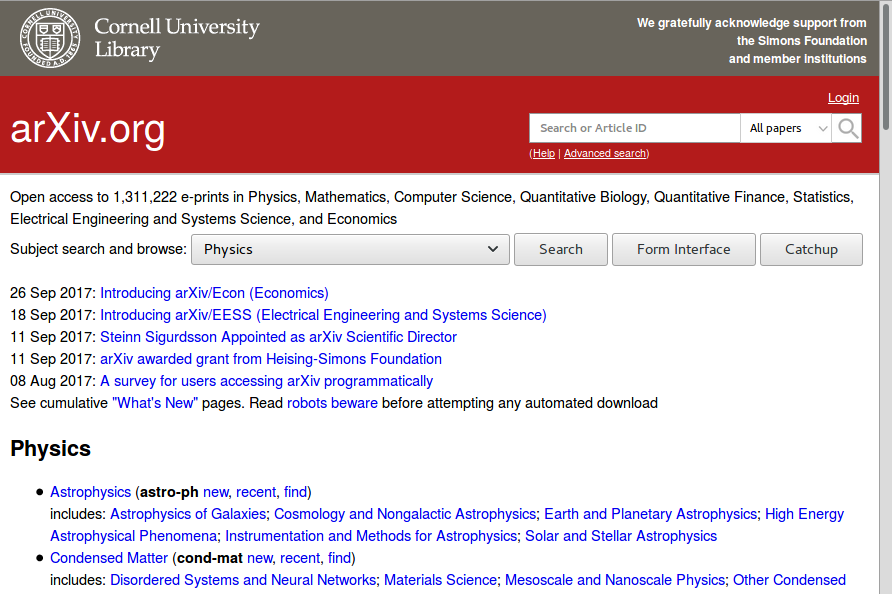
\includegraphics{site}
\end{frame}

\begin{frame}{Общий вид сайта}
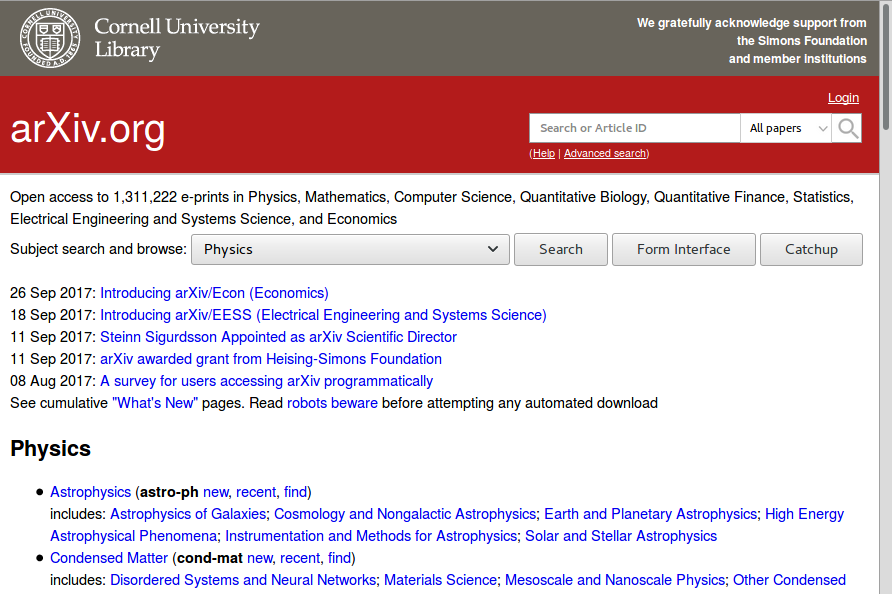
\includegraphics[width=\linewidth]{site}
\end{frame}

\begin{frame}{Computer Science}
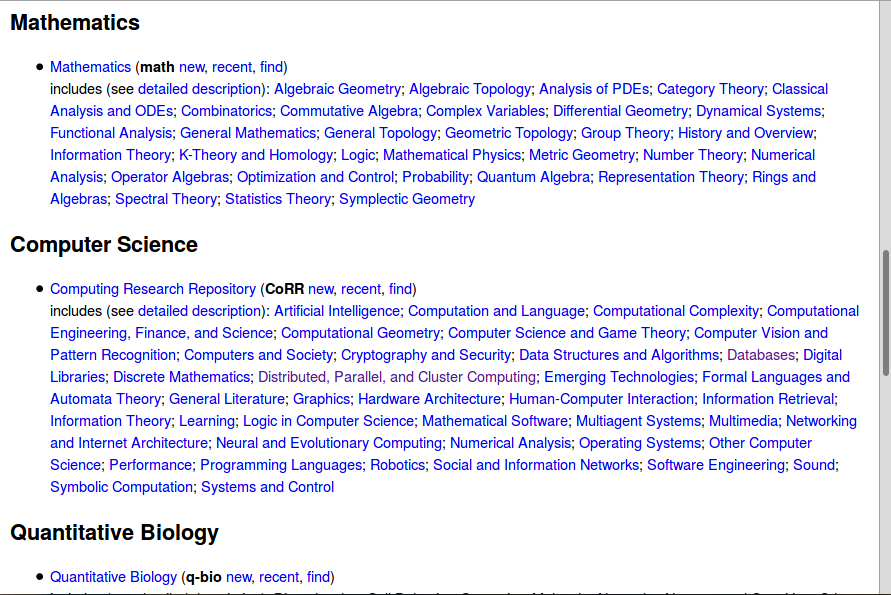
\includegraphics[width=\linewidth]{computer_science}
\end{frame}

\begin{frame}{Computer Science}
Artificial Intelligence (Искусственный интеллект)

Computation and Language (Вычисления и языки)

Computational Complexity (Вычислительная сложность)

Computational Engineering, Finance, and Science (Вычислительная инженерия, финансы и наука)

Computational Geometry (Вычислительная геометрия)

Computer Science and Game Theory (Компьютерные науки и теория игр)
\end{frame}

\begin{frame}{Computer Science}
Computer Vision and Pattern Recognition (Компьютерное зрение и распознавание образов)

Computers and Society (Компьютеры и общество)

Cryptography and Security (Шифрование и безопасность)

Data Structures and Algorithms (Структуры данных и алгоритмы)

Databases (Базы данных)
\end{frame}

\begin{frame}{Computer Science}
Digital Libraries (Цифровые библиотеки)

Discrete Mathematics (Дискретная математика)

Distributed, Parallel, and Cluster Computing (Распределённые, параллельные и кластерные вычисления)

Emerging Technologies (Новые, перспективные и инновационные технологии)
\end{frame}

\begin{frame}{Computer Science}
Formal Languages and Automata Theory (Формальные языки и теория автоматов)
 
General Literature (Общая литература)

Graphics (Графика)

Hardware Architecture (Аппаратная архитектура)

Human-Computer Interaction (Человеко-машинное взаимодействие)
\end{frame}

\begin{frame}{Computer Science}
Information Retrieval (Информационный поиск)

Information Theory (Теория информации)

Learning (Машинное обучение)

Logic in Computer Science (Логика в компьютерных науках)

Mathematical Software (Математическое программное обеспечение)
\end{frame}

\begin{frame}{Computer Science}
Multiagent Systems (Мультиагентные системы)

Multimedia (Мультимедиа)

Networking and Internet Architecture (Сети и архитектура Интернета)

Neural and Evolutionary Computing (Нейронные и эволюционные вычисления)

Numerical Analysis (Численный анализ)

Operating Systems (Операционные системы)
\end{frame}

\begin{frame}{Computer Science}
Other Computer Science (Другое в компьютерных науках)

Performance (Высокопроизводительные вычисления)

Programming Languages (Языки программирования)

Robotics (Робототехника)

Social and Information Networks (Социальные и информационные сети)
\end{frame}

\begin{frame}{Computer Science}
Software Engineering (Программная инженерия)

Sound (Звук)

Symbolic Computation (Символьные вычисления)

Systems and Control (Системы и управление)
\end{frame}

\begin{frame}{Смежные области}
Physics

Mathematics

Quantitative Biology

Quantitative Finance

Statistics

Electrical Engineering and Systems Science

Economics
\end{frame}

\begin{frame}{История}
Проект был создан в августе 1991 года в Лос-Аламосской национальной лаборатории и предназначался для публикации статей по физике.

На данный момент поддерживается Корнеллским университетом и является частью его библиотеки.
\end{frame}

\begin{frame}{Цитирование и рецензирование}
Публикуемые статьи автоматически добавлялись в базу цитирования Citebase. Но эта база на данный момент уже не функционирует.

Публикуемые статьи не проходят научное рецензирование, однако в 2004 году была введена процедура поручительства, при этом при наличии статуса поручителя можно публиковать статью без поручительства.
\end{frame}

\begin{frame}{Статистика}
На 5 октября число подключений составляло от 150 тыс. до 200 тыс. в час.

Общее число подключений составило около 3 млн.

Число загрузок в целом из года в год растёт, и в 2016 году достигло пика в 6 млн.
\end{frame}

\begin{frame}{Статистика}
Пользователями являются представители таких известных организаций и университетов как: CERN, Токийский университет, Центр Макса-Планка, Университет Кембриджа, MIT, Berkeley, ETH Zurich, Принстонский университет, Университет Киото, Оксфорд, Колумбийский университет.
\end{frame}

\begin{frame}{Статистика}
Среди Топ-200 пользователей, к сожалению, не обнаружены ни МГУ, ни ИТМО, ни СПбГУ.
\end{frame}

\begin{frame}{Статистика}
Число загружаемых в архив статей также растёт из года в год и в сентябре 2017 составило 10 тыс.

Общее число статей на 5 октября 2017 составляет 1 млн. 311 тыс. 222.
\end{frame}

\begin{frame}{Статистика}
Примерно половина всех загружаемых в архив статей являются статьи по различным областям физики. Однако из года в год растёт число публикаций в области математики (примерно четверть) и компьютерных наук (примерно пятая часть). На остальные представленные в архиве науки приходится суммарно около 5\%.
\end{frame}

\begin{frame}{Особенности публикации}
Большинство публикаций представлены в формате \TeX, а также в автоматически генерируемых из него форматах PDF и PostScript. Также могут быть представлены в форматах PDF, PostScript и HTML.

Изображения должны быть представлены в форматах PS/EPS, JPEG, GIF, PNG, PDF.
\end{frame}

\begin{frame}{Особенности публикации}
Публикации принимаются только от зарегистрированных авторов. Регистрироваться нужно только, если планируется публикация в архиве.

Авторы предоставляют статьи под non-exclusive and irrevocable license to distribute (неисключительные и безотзывные права для распространения).
\end{frame}

\begin{frame}{Представление статьи}
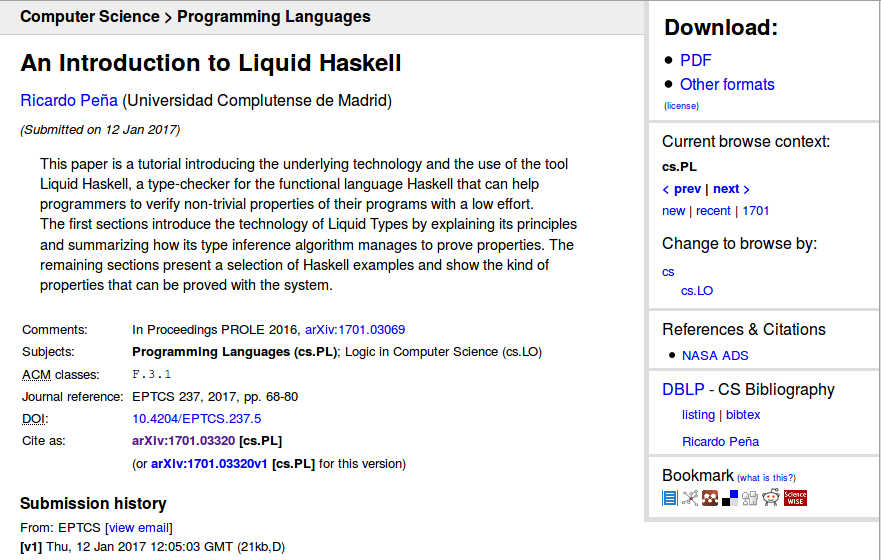
\includegraphics[width=\linewidth]{article_page}
\end{frame}

\begin{frame}{Машинный доступ}
Не нужно осуществлять crawling. Архив предоставляет несколько способов машинного чтения: OAI-PMH (\url{http://www.openarchives.org/}), API, RSS.
\end{frame}

\begin{frame}{Ответы на вопросы}
\url{https://arxiv.org/help/support/faq}
\end{frame}

\begin{frame}[nologo]
\centering\textit{Ни один котик не пострадал.}
\end{frame}

\itmothankyou

\end{document}

